\documentclass[12pt,a4paper]{article}
\usepackage[utf8]{inputenc}
\usepackage[T1]{fontenc}
\usepackage[spanish]{babel}

\usepackage{amsmath}
\usepackage{amssymb}

\usepackage{graphicx}
\usepackage{float}

\usepackage{geometry}
\geometry{
left=2.5cm,
right=2.5cm,
top=2.5cm,
bottom=2.5cm
}

\begin{document}

\begin{titlepage}
\centering
\vspace*{2cm}

{\Large\textbf{Tarea 01}\par}

\vspace{0.5cm}
\rule{10cm}{0.5pt}

\vspace{1.5cm}

{\LARGE\textbf{Análisis en el tiempo de SLID}\par}

\vspace{0.5cm}
\rule{10cm}{0.3pt}

\vspace{2cm}

{\Large Procesamiento Digital de Señales\par}

\vspace{0.3cm}
{\large Maestría en Procesamiento de Señales\par}
{\large UNAM, 2026-1\par}

\vfill

\vspace{2cm}

{\Large\textbf{Autor:}\par}
{\large Angel Miguel Hernandez Abarca\par}

\vspace{2cm}

\end{titlepage}

% ==================== EJERCICIO 1 ====================
\newpage
\section*{Ejercicio 1}

Escriba un programa en Matlab u Octave que realice lo siguiente:

\begin{itemize}
\item Generar una señal $x_a(t)$ con dos componentes frecuenciales $f_1 \ll f_2$.
\item Tomar muestras de esta señal con $f_{s1} < f_2$ y con $f_{s2} > f_2$.
\item Reconstruir la señal original mediante la función de interpolación
\begin{equation}
g(t) = \frac{\sin 2\pi B t}{2\pi B t}
\end{equation}
\item Graficar la señal original y la reconstruida, con ambas frecuencias de muestreo, y comparar.
\end{itemize}

Grafica de la señal original y la reconstruida con ambas frecuencias de muestreo:
\vspace{0.6cm}

\begin{figure}[H]
\centering
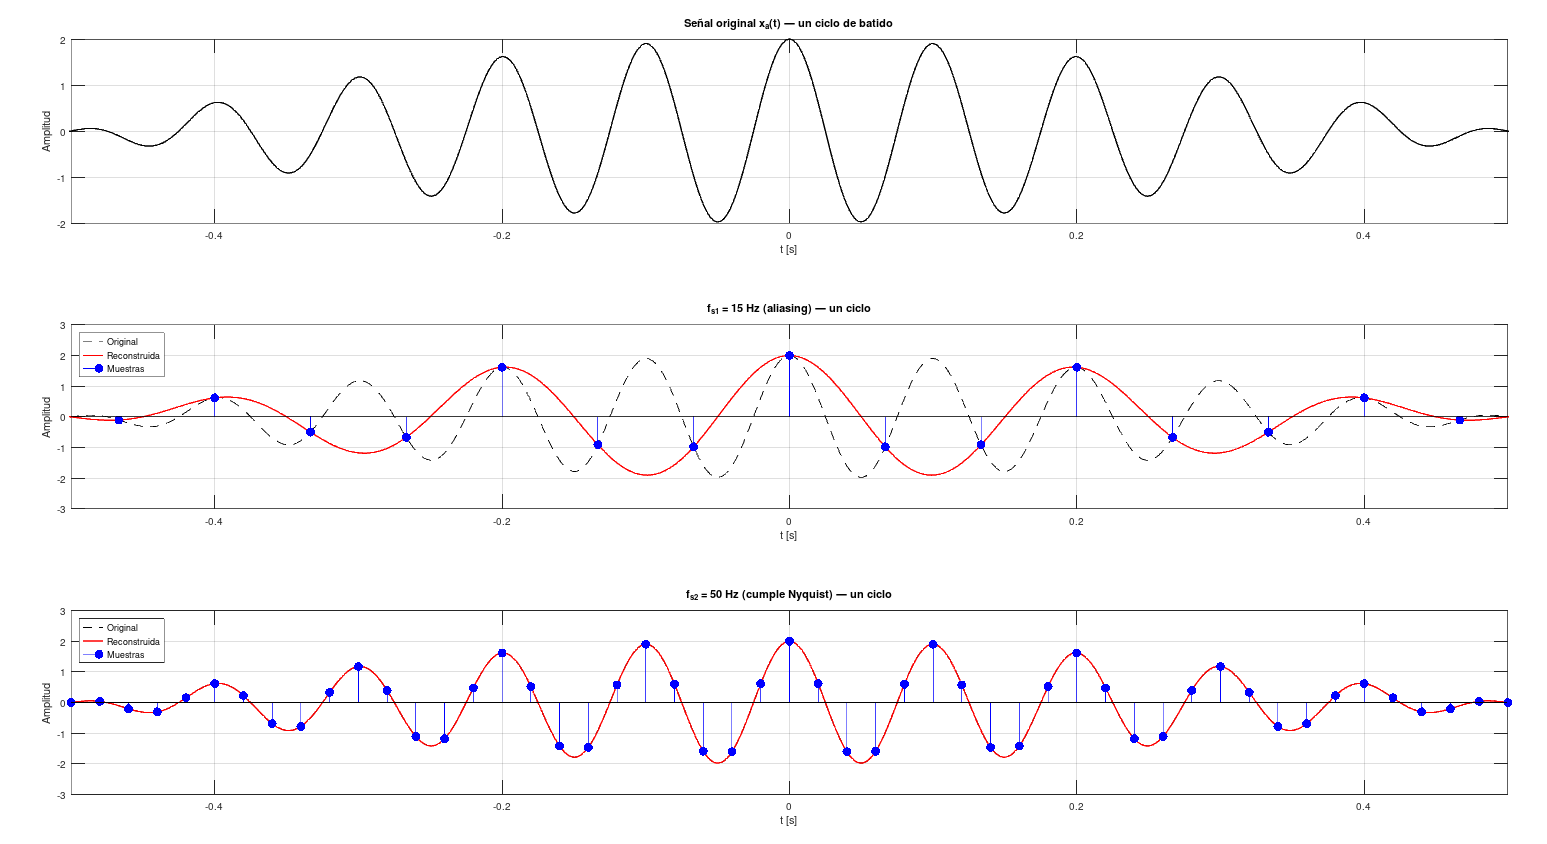
\includegraphics[width=1.0\textwidth]{Graficas.png}
\end{figure}
% ==================== EJERCICIO 2 ====================
\newpage
\section*{Ejercicio 2}

Para cada sistema, determine si es estatico o dinamico, lineal o no lineal, variante o invariante ante el desfase,
causal o no causal.

\begin{itemize}
\item \textbf{Estático/Dinámico:} Un sistema es Estático si la salida $y(n)$ solo depende de la entrada en el mismo tiempo $x(n)$ y 
no depende de muestras pasadas ni futuras. En cualquier otro caso, se dice que el sistema es Dinámico.
\item \textbf{Lineal/No lineal:} Un sistema es lineal si cumple con homogeneidad y aditividad.
\item \textbf{Invariante/Variante:} Un sistema es invariante ante el desfase si se cumple que: Si $x(n) \to x(n-n_0)$, entonces $y(n) \to y(n-n_0)$.
\item \textbf{Causal/No causal:} Un sistema discreto es causal, si la salida y(n) se puede obtener conociendo solo la entrada actual x(n) y
entradas anteriores, es decir, $y(n)$ depende de $x(n)$ y de $x(n-k)$ con $k \geq 0$. En cualquier otro caso, se dice que el sistema es No causal.
\end{itemize}

\subsection*{a) $y(n) = \cos[x(n)]$}

\begin{itemize}
\item \textbf{Estático:} Solo usa $x(n)$, el instante actual.
\item \textbf{No lineal:} Dado que no cumple con el teorema de superposición
\item \textbf{Invariante:} Si $x(n) \to x(n-n_0)$, la salida es $\cos[x(n-n_0)] = y(n-n_0)$. No hay dependencia explícita de $n$ fuera de $x$.
\item \textbf{Causal:} Solo usa el presente.
\end{itemize}

\subsection*{b) $y(n) = x(n)\cos(\omega n)$}

\begin{itemize}
\item \textbf{Estático:} Solo $x(n)$.
\item \textbf{Lineal:} Dado que se cumple el teorema de superposición: $T[ax_1 + bx_2] = (ax_1(n) + bx_2(n))\cos(\omega n) = aT[x_1] + bT[x_2]$.
\item \textbf{Variente:} El sistema es variante ante el desfase ya que cumple con $x(n) \to x(n-n_0)$, la salida es $y(n) = x(n-n_0)\cos(\omega n)$
\item \textbf{Causal:} Solo presente.
\end{itemize}

\subsection*{c) $y(n) = x(-n+2)$}

\begin{itemize}
\item \textbf{Dinámico:} Para obtener $y(n)$ necesitas $x$ evaluada en $-n+2$, que en general es un instante distinto (pasado o futuro) de $n$.
\item \textbf{Lineal:} Dado que se cumple el teorema de superposición: $T[ax_1 + bx_2] = (ax_1(n) + bx_2(n))\cos(\omega n) = aT[x_1] + bT[x_2]$.
\item \textbf{Variante:} El sistema es variante ya que cumple con $x(n) \to x(n-n_0)$, la salida es $y(n) = x(-n+2-n_0)$, que no es igual a $y(n-n_0) = x(-n+n_0+2)$.
\item \textbf{No causal:} Por ejemplo, para $n=0$, $y(0) = x(2)$, que es una muestra futura respecto a $n=0$.
\end{itemize}

\subsection*{d) $y(n) = |x(n)|$}

\begin{itemize}
\item \textbf{Estático:} Solo presente.
\item \textbf{No lineal:} El valor absoluto no es aditivo ($|x_1 + x_2| \neq |x_1| + |x_2|$ en general, ej. $x_1 = 1, x_2 = -1$).
\item \textbf{Invariante:} La regla ``toma valor absoluto'' no depende de $n$.
\item \textbf{Causal:} Solo presente.
\end{itemize}

\subsection*{e) $y(n) = x(n)u(n)$}

\begin{itemize}
\item \textbf{Estático:} Solo presente.
\item \textbf{Lineal:} Dado que cumple con el teorema de superposición: $T[ax_1 + bx_2] = (ax_1(n) + bx_2(n))u(n) = aT[x_1] + bT[x_2]$.
\item \textbf{Variante:} Dado que cumple con $x(n) \to x(n-n_0)$, la salida es $y(n) = x(n-n_0)u(n)$, que no es igual a $y(n-n_0) = x(n-n_0)u(n-n_0)$.
\item \textbf{Causal:} Solo presente, aunque multiplicado por 0 en $n < 0$.
\end{itemize}

\subsection*{f) $y(n) = x(n) + x(n-1)$}

\begin{itemize}
\item \textbf{Dinámico:} Usa el presente y una muestra pasada.
\item \textbf{Lineal:} Suma de dos operaciones lineales.
\item \textbf{Invariante:} Entrada retrasada: $x(n-n_0) + x(n-1-n_0)$; y $y(n-n_0) = x(n-n_0) + x(n-n_0-1)$ — son idénticos. (Invariante)
\item \textbf{Causal:} Usa $n$ y $n-1 \leq n$.
\end{itemize}

\subsection*{g) $y(n) = x(2n)$}

\begin{itemize}
\item \textbf{Dinámico:} Accede a muestras en diferentes instantes.
\item \textbf{Lineal:} Es válida la superposición.
\item \textbf{Invariante:} Dado que no cumple con $x(n) \to x(n-n_0)$ el sistema es invariante ante el desfase.
\item \textbf{No causal:} Dado que la salida actual depende de salidas futuras, el sistema es no causal.
\end{itemize}

\subsection*{h) $y(n) = x(-n)$}

\begin{itemize}
\item \textbf{Dinámico:} Dado que la salida actual depende de muestras pasadas de la señal de entrada, $y(n)$ es un sistema
\item \textbf{Lineal:} Es válida la superposición.
\item \textbf{Variante:} Dado que no cumple con $x(n) \to x(n-n_0)$ el sistema es variante ante el desfase.
\item \textbf{No causal:} Para $n < 0$ se necesita $x$ en un índice positivo, es decir ``futuro'' relativo.
\end{itemize}

\subsection*{i) $y(n) = \text{sign}[x(n)]$}

\begin{itemize}
\item \textbf{Estático:} Solo presente.
\item \textbf{No lineal:} Dado que no cumple con el teorema de superposición.
\item \textbf{Invariante:} La regla no depende de $n$.
\item \textbf{Causal:} Solo presente.
\end{itemize}


% ==================== EJERCICIO 3 ====================
\section*{Ejercicio 3}

Considere un sistema discreto G cuya respuesta al impulso está dada por:

\begin{equation}
h(n) = \delta(n) + 2\delta(n-1)
\end{equation}

La salida $y(n)$ cuando la entrada es $x(n) = \{0, 2, 3\}$.

\textbf{Convolución:}

\begin{equation}
y(n) = x(n) * h(n)
\end{equation}

\textbf{Convolución:}

\begin{equation}
\boxed{y(n) = \{0, \underline{0}, 2, 7, 6, 0, \ldots\}}
\end{equation}

% ==================== EJERCICIO 4 ====================
\section*{Ejercicio 4}

Calcule la convolución de:
\vspace{0.4cm}

\subsection*{a) $x(n) = (1/2)^n u(n)$ y $h(n) = \{1, -1\}$}
\vspace{0.4cm}

Aplicando el metodo de la regleta se obtiene:
\vspace{0.4cm}

\begin{equation}
\boxed{x(n) = \{0, \underline{1}, -1/2, -1/4, -1/8 \ldots\}}
\end{equation}
\vspace{0.4cm}

\subsection*{b) $x(n) = \delta(n)$ + 0.5 $\delta(n-1)$ y $h(n) = u(n)$}
\vspace{0.4cm}

Aplicando el metodo de la regleta se obtiene:
\vspace{0.4cm}

\begin{equation}
\boxed{x(n) = \{0, \underline{1}, 3/2, 3/2, 3/2, 3/2, \ldots\}}
\end{equation}
\vspace{0.4cm}

\subsection*{c) $x(n) = a^n u(n)$ y $h(n) = b^n u(n)$}
\vspace{0.4cm}

Para a=b y para a $\neq$ b, se tiene:
\vspace{0.4cm}

\begin{equation}
y(n) = \sum_{k=-\infty}^{\infty} x(k) * h(n-k)
\end{equation}


Dicho lo anterior ambas señales coexisten en $0 \leq k \leq n$, entonces:

\begin{equation}
y(n) = \left(\sum_{k=0}^{n} a^k u(k) b^{n-k}\right) u(n-k)
\end{equation}

Factorizamos $b^n$:

\begin{equation}
y(n) = b^n \sum_{k=0}^{n} \left(\frac{a}{b}\right)^k u(n)
\end{equation}
\vspace{0.4cm}

Para $a = b$:

\begin{equation}
y(n) = a \sum_{k=0}^{n} 1
\end{equation}
\vspace{0.4cm}

\begin{equation}
\boxed{y(n) = a^n(n+1) u(n)}
\end{equation}



Entonces, para $a \neq b$:

\begin{equation}
y(n) = b^n \frac{1-(a/b)^{n+1}}{1-(a/b)} u(n)
\end{equation}

\begin{equation}
\boxed{y(n) = \frac{a^{n+1} - b^{n+1}}{a - b} u(n)}
\end{equation}

% ==================== EJERCICIO 5 ====================
\section*{Ejercicio 5}

Considere un sistema SLID y se conoce la respuesta al escalón $S(n)$. Exprese la respuesta al impulso $h(n)$ en términos del escalón.

Donde:

\begin{equation}
S(n) = h(n) * u(n)
\end{equation}

\begin{equation}
S(n) = \sum_{k=-\infty}^{\infty} u(n-k)h(k)
\end{equation}

\textbf{Escalón:}

\begin{equation}
u(x) = \begin{cases}
0 & x < 0 \\
1 & x \geq 0
\end{cases}
\end{equation}

\begin{equation}
S(n) = \sum_{k=0}^{n} h(k)
\end{equation}

Entonces:

\begin{equation}
S(n) - S(n-1) = \sum_{k\leq n} h(k) - \sum_{k\leq n-1} h(k) = h(n)
\end{equation}

\begin{equation}
S(n) - S(n-1) = h(n) \quad \Rightarrow  \boxed{\quad h(n) = S(n) - S(n-1)}
\end{equation}

% ==================== EJERCICIO 6 ====================
\section*{Ejercicio 6}

Considere una señal  $\lambda(n)$ = $a^n u(n)$
\vspace{0.4cm}

con: 0 < a < 1 
\vspace{0.4cm}

Demuestre que toda señal $x(n)$ se puede expresar en: 

\begin{equation}
x(n) = \sum_{k=-\infty}^{\infty} c_k \lambda(n-k)
\end{equation}

En términos del escalón $\lambda(n)$:

\begin{equation}
\lambda(n) = a^n u(n)
\end{equation}

\begin{equation}
\lambda(n-1) = a^{n-1} u(n-1)
\end{equation}

\begin{equation}
a \lambda(n-1) = a^n u(n-1)
\end{equation}

Aislar el impulso:

\begin{equation}
\lambda(n) - a \lambda(n-1) = a^n(u(n) - u(n-1))
\end{equation}
\newpage

Entonces:

\begin{equation}
u(n) - u(n-1) = \delta(n)
\end{equation}

\begin{equation}
\delta(n) = \lambda(n) - a \lambda(n-1)
\end{equation}

Una señal discreta está dada por:

\begin{equation}
x(n) = \sum_{k=-\infty}^{\infty} x(k) \delta(n-k)
\end{equation}

Al sustituir $\delta(n-k)$:

\begin{equation}
x(n) = \sum_{k=-\infty}^{\infty} x(k)(\lambda(n-k) - a \lambda(n-k-1))
\end{equation}

\begin{equation}
x(n) = \sum_{k=-\infty}^{\infty} x(k)\lambda(n-k) - \sum_{k=-\infty}^{\infty} a x(k)\lambda(n-k-1)
\end{equation}

\begin{equation}
x(n) = \sum_{k=-\infty}^{\infty} (x(k) - a x(k-1)) \lambda(n-k)
\end{equation}

Por lo tanto:

\begin{equation}
x(n) = \sum_{k=-\infty}^{\infty} c_k \lambda(n-k)
\end{equation}

donde:

\begin{equation}
\boxed{c_k = x(k) - a x(k-1)}
\end{equation}

% ==================== EJERCICIO 7 ====================
\section*{Ejercicio 7}

Considere un SLID y la señal $\lambda(n)$ del inciso anterior. Considere que se conoce la salida $g(n)$ 
para la señal $\gamma(n)$. Exprese la respuesta al impulso en terminos de la señal $g(n)$.

\begin{equation}
\lambda(n) = a^n u(n)
\end{equation}

Con superposición, entonces:

\begin{equation}
x(n) = x(n) * h(n) \quad ; \quad g(n) = \lambda(n) * h(n)
\end{equation}

\begin{equation}
h(n) = h(n) * (\lambda(n) - a \lambda(n-1))
\end{equation}

\begin{equation}
h(n) = (h(n) * \lambda(n)) - (h(n) * a \lambda(n-1))
\end{equation}

\begin{equation}
h(n) * a \lambda(n-1) = a g(n-1)
\end{equation}

\begin{equation}
\boxed{h(n) = g(n) - a g(n-1)}
\end{equation}

% ==================== EJERCICIO 8 ====================
\section*{Ejercicio 8}

Considere el sistema:

\begin{equation}
y(n) - y(n-1) + \frac{1}{2} y(n-2) = x(n)
\end{equation}

Determine el escalón. $X(n) = u(n)$
\vspace{0.4cm}

donde:

\begin{equation}
u(n) = \begin{cases}
0 & n \geq 0 \\
1 & n < 0
\end{cases}
\end{equation}

Sustituimos:

\begin{equation}
y(n) - y(n-1) + \frac{1}{2} y(n-2) = u(n)
\end{equation}

Ecuación homogénea, se propone $y(n) = r^n$:

\begin{equation}
y(n) = y(n-1) + \frac{1}{2} y(n-2) + x(n)
\end{equation}
\vspace{0.4cm}

despues de dividir entre $r^{n-2}$:
\begin{equation}
r^2 - r + \frac{1}{2} = 0
\end{equation}
\vspace{0.4cm}

Fórmula general:

\begin{equation}
r = \frac{1 \pm \sqrt{1-2}}{2} = \frac{1 \pm j}{2}
\end{equation}

Entonces $r = \frac{1}{\sqrt{2}} e^{j\pi/4}$, $r = \left(\frac{1}{\sqrt{2}}\right)^j\left(\frac{1}{\sqrt{2}}\right)^j$
\vspace{0.4cm}

La solución homogénea:

\begin{equation}
y(n) = \left(\frac{1}{\sqrt{2}}\right)^n \left(c_1 \cos\left(\frac{\pi n}{4}\right) + c_2 \sin\left(\frac{\pi n}{4}\right)\right)
\end{equation}

Solución particular: 

\begin{equation}
y(n) = k
\end{equation}


Sustituyendo: 
\begin{equation}
k - k + \frac{1}{2} k = 1 \Rightarrow k = 2
\end{equation}


\begin{equation}
y(n) = 2 + \left(\frac{1}{\sqrt{2}}\right)^n \left(c_1 \cos\left(\frac{\pi n}{4}\right) + c_2 \sin\left(\frac{\pi n}{4}\right)\right)
\end{equation}
\vspace{0.4cm}

$y(0) = 1$

\begin{equation}
1 = 2 + C_1 \Rightarrow c_1 = 1 - 2
\end{equation}
\begin{equation}
\boxed{c_1 = -1}
\end{equation}

\begin{equation}
c_1 = 1 - 2 = -1
\end{equation}

$y(n) = 2$

\begin{equation}
2 = 2 + \left(\frac{1}{\sqrt{2}}\right)\left(-1\cos\left(\frac{\pi}{4}\right) + c_2 \sin\left(\frac{\pi}{4}\right)\right)
\end{equation}

$\cos \frac{\pi}{4} = \sin \frac{\pi}{4} = \frac{1}{\sqrt{2}}$:

\begin{equation}
0 = \frac{1}{\sqrt{2}} \left(-\frac{1}{2} + \frac{c_2}{\sqrt{2}}\right) \Rightarrow \boxed{c_2 = 1}
\end{equation}

\begin{equation}
\boxed{y(n) = 2 + \left(\frac{1}{\sqrt{2}}\right)^n \left(\cos\left(\frac{\pi n}{4}\right) + \sin\left(\frac{\pi n}{4}\right)\right) u(n)}
\end{equation}

% ==================== EJERCICIO 9 ====================

\section*{Ejercicio 9}

Considere $x(n) = a^n u(n)$ con $0 < a < 1$.

\subsection*{a) Energía $E_x$ de $x(n)$}

\begin{equation}
E_x = \sum_{n=-\infty}^{\infty} |x(n)|^2 
\end{equation}

\begin{equation}
u(n) = \begin{cases}
0 & n \geq 0 \\
1 & n < 0
\end{cases}
\end{equation}

\begin{equation}
E_x = \sum_{n=-\infty}^{\infty} |a|^{2n} u(n) \Rightarrow  \sum_{n=-\infty}^{\infty} a^{2n}
\end{equation}

\textbf{Serie geométrica:}

\begin{equation}
\sum_{n=0}^{\infty} r^n = \frac{1}{1 - r^n} \quad ; \quad \sum_{n=0}^{\infty} a^{2n} = \boxed{\frac{1}{1-a^2}}
\end{equation}

\subsection*{b) Expresión analítica para la autocorrelación $r_{xx}(n)$ de $x(n)$}

\begin{equation}
r_{xx} = \sum_{k=-\infty}^{\infty} x(n+k) x(n)
\end{equation}

\begin{equation}
r_{xx} = \sum_{k=-\infty}^{\infty} a^n u(n) a^{n-k} u(n-k)
\end{equation}

Entonces:

\begin{equation}
r_{xx} = \sum_{k=-\infty}^{\infty} a^{2n-k} u(n) u(n-k)
\end{equation}

\begin{equation}
r_{xx} = \sum_{n=k}^{\infty} a^{2n-k} \quad ; \quad a^{2n-k} = a^{-k} a^{2n}
\end{equation}

\begin{equation}
r_{xx} = a^{-k} \sum_{n=k}^{\infty} a^{2n} \quad ; \quad r_{xx}(k) = \boxed{\frac{a^k}{1-a^2}}
\end{equation}

% ==================== EJERCICIO 10 ====================
\section*{Ejercicio 10}

Determine la autocorrelación de $x(n) = \sin(wn)$.

\begin{equation}
r_{xx}(k) = \lim_{N \to \infty} \frac{1}{2M+1} \sum_{n=-M}^{M} x(n) x(n-k)
\end{equation}

Donde:

\begin{equation}
x(n) = \sin(wn)
\end{equation}

\begin{equation}
x(n-l) = \sin(w(n-l))
\end{equation}

\begin{equation}
r_{xx}(k) = \lim_{N \to \infty} \frac{1}{N} \sum_{n=0}^{N-1} \sin(wn) \sin(w(n-k))
\end{equation}

Por identidad trigonométrica:

\begin{equation}
\sin(wn) \sin(wn+wk) = \frac{1}{2} \cos(-wk) - \frac{1}{2} \cos(2wn+wk) = \frac{1}{2}\cos(wk) - \frac{1}{2}\cos(2wn+wk)
\end{equation}

\begin{equation}
r_{xx}(k) = \lim_{N \to \infty} \frac{1}{N} \sum_{n=0}^{N-1} \frac{1}{2}\cos(wk) - \cos(2wn+wk)
\end{equation}

\begin{equation}
r_{xx}(k) = \frac{1}{2}\lim_{N \to \infty} \frac{1}{N} \sum_{n=0}^{N-1}\cos(wk) - \cos(2wn+wk)
\end{equation}

\begin{equation}
r_{xx}(k) = \frac{1}{2} \left[\left(\lim_{N \to \infty} \frac{1}{N} \sum_{n=0}^{N-1} \cos(wk)\right) - \left(\lim_{N \to \infty} \frac{1}{N} \sum_{n=0}^{N-1} \cos(2wn+wk)\right)\right]
\end{equation}

Donde:

\begin{equation}
\lim_{N \to \infty} \frac{1}{N} \sum_{n=0}^{N-1} \cos(wk) = \boxed{\cos(wk)}
\end{equation}

\begin{equation}
\lim_{N \to \infty} \frac{1}{N} \sum_{n=0}^{N-1} \cos(2wn+wk) = \boxed{0}
\end{equation}

Por lo tanto:

\begin{equation}
r_{xx}(k) = \frac{1}{2} \cos(wk) - 0 \Rightarrow {r_{xx}(k) = \frac{1}{2} \cos(wk)}
\end{equation}

\begin{equation}
\boxed{r_{xx}(k) = \frac{1}{2} \cos(wn)}
\end{equation}
\end{document}